%%%%%%%%%%%%%%%%%%%% author.tex %%%%%%%%%%%%%%%%%%%%%%%%%%%%%%%%%%%
%
% sample root file for your "contribution" to a contributed volume
%
% Use this file as a template for your own input.
%
%%%%%%%%%%%%%%%% Springer %%%%%%%%%%%%%%%%%%%%%%%%%%%%%%%%%%


% RECOMMENDED %%%%%%%%%%%%%%%%%%%%%%%%%%%%%%%%%%%%%%%%%%%%%%%%%%%
\documentclass[graybox]{svmult}

% choose options for [] as required from the list
% in the Reference Guide

\usepackage{type1cm}        % activate if the above 3 fonts are
                            % not available on your system
%
\usepackage{makeidx}         % allows index generation
\usepackage{graphicx}        % standard LaTeX graphics tool
                             % when including figure files
\usepackage{multicol}        % used for the two-column index
\usepackage[bottom]{footmisc}% places footnotes at page bottom


\usepackage{newtxtext}       % 
\usepackage{newtxmath}       % selects Times Roman as basic font

% see the list of further useful packages
% in the Reference Guide

\makeindex             % used for the subject index
                       % please use the style svind.ist with
                       % your makeindex program

%%%%%%%%%%%%%%%%%%%%%%%%%%%%%%%%%%%%%%%%%%%%%%%%%%%%%%%%%%%%%%%%%%%%%%%%%%%%%%%%%%%%%%%%%

%=========================Manage Comments=============================
\usepackage{color}
\usepackage{ifthen}
\newboolean{showcomments}
\setboolean{showcomments}{true} % toggle to show or hide comments
\ifthenelse{\boolean{showcomments}}
    {
        \newcommand{\emelie}[1]{\textcolor{red}{{\it [Emelie says: #1]}}}
        \newcommand{\peggy}[1]{\textcolor{blue}{{\it [Peggy says: #1]}}}
        \newcommand{\per}[1]{\textcolor{cyan}{{\it [Per says: #1]}}}
         \newcommand{\cassie}[1]{\textcolor{gray}{{\it [Cassie says: #1]}}}
        \newcommand{\othercomment}[1]{\textcolor{magenta}{{\it [#1]}}}
    }
    {
        \newcommand{\emelie}[1]{}
        \newcommand{\peggy}[1]{}
        \newcommand{\per}[1]{}
        \newcommand{\cassie}[1]{}
        \newcommand{\othercomment}[1]{}
    }
%=======================================================================

%(1)    The formatting templates (in both LaTeX and Word) are available under [1]. The current LaTeX template is directly available at [2] (please use the template from the subdirectory “author” in the zip file) and the current Word template at [3].
%(2)    The chapters should be written in a clear, consistent, self-contained textbook-like style. Therefore, please comply with the following structure:
%a.       Each chapter should start with an “Introduction” and end with a short “Conclusion”. Please also consider a section “Recommended Further Reading” before the Conclusion.
%b.       The goal of each chapter is to give a comprehensive overview on a contemporary topic in empirical software engineering (for your convenience you find below a list of the confirmed chapter topics)
%c.       Please provide examples and evidence
%(3)    The intended length of your chapter should be approximately 25 pages.
%(4)    The deadline to submit the first version of the chapter is the 30th of April 2019.



\begin{document}

\title*{The Design Science Paradigm as a Frame for Empirical Software Engineering}
% Use \titlerunning{Short Title} for an abbreviated version of
% your contribution title if the original one is too long
\author{Per Runeson, Emelie Engstr\"om and Margaret-Anne Storey}
% Use \authorrunning{Short Title} for an abbreviated version of
% your contribution title if the original one is too long
\institute{Per Runeson and Emelie Engstr\"om \at Lund University, Sweden, \email{[per.runeson;emelie.engstrom]@cs.lth.se}
\and Margaret-Anne Storey \at University of Victoria, Canada, \email{mstorey@uvic.ca}}
%
% Use the package "url.sty" to avoid
% problems with special characters
% used in your e-mail or web address
%
\maketitle
\abstract*{Each chapter should be preceded by an abstract (no more than 200 words) that summarizes the content. The abstract will appear \textit{online} at \url{www.SpringerLink.com} and be available with unrestricted access. This allows unregistered users to read the abstract as a teaser for the complete chapter.
Please use the 'starred' version of the \texttt{abstract} command for typesetting the text of the online abstracts (cf. source file of this chapter template \texttt{abstract}) and include them with the source files of your manuscript. Use the plain \texttt{abstract} command if the abstract is also to appear in the printed version of the book.}

\abstract{Software engineering research aims to help improve real-world practice. With the adoption of empirical software engineering research methods, the understanding of real-world needs and validation of solution proposals have evolved. However, the philosophical perspective on what constitutes theoretical knowledge and research contributions in software engineering is less discussed in the community.   In this chapter, we use the \emph{design science paradigm} as a frame for articulating and communicating prescriptive software engineering research contributions. 
Design science embraces \emph{problem conceptualization, solution (or artifact) design}, and \emph{validation} of solution proposals, with recommendations for practice phrased as \emph{technological rules}. Design science is used in related research areas, particularly information systems and management theory. We elaborate the constructs of design science for software engineering, relate them to different conceptualizations of design science and provide examples of possible research methods. We outline how the assessment of research contributions, industry-academia communication and theoretical knowledge building may be supported by the design science paradigm. Finally, we provide examples of software engineering research presented through a design science lens.} 
\per{I use frame for the general discussion and lens for the VA. ok?}

\section{Introduction}
\label{sec:intro}

%In the beginning...
Software engineering research aims to develop and validate practically useful methods, technologies, and tools to help industry improve software engineering practice. This practical aspect was discussed when the term `software engineering' was coined by Margaret Hamilton in the late 1960s\footnote{https://publications.computer.org/software-magazine/2018/06/08/margaret-hamilton-software-engineering-pioneer-apollo-11/}, and later put in print in a NATO conference report~\cite{Nato1968}. 

\begin{quote}
{The phrase `software engineering'  [implied] the need for software manufacture to be based on the types of theoretical foundations and practical disciplines that are traditional in the established branches of engineering}~\cite[p. 13]{Nato1968}. 
\end{quote}

Numerous solutions to software engineering problems have been proposed and published during the past few decades---these include development methods and processes, tools, frameworks, taxonomies, or languages---but few involve systematic investigations of real-world problem instances and validation by large-scale software practice.

%Empirical software engineering
With the advent of empirical software engineering~\cite{Basili86} and evidence-based software engineering~\cite{Kitchenham04}, the research focus has shifted towards an empirically informed understanding of practice and solution proposals. Empirical methods have been inherited and adapted from other research fields, particularly medicine and the social sciences. Applying these methods, the software engineering knowledge base has been systematically extended through families of experiments~\cite{Basili99} and systematic literature reviews~\cite{Kitchenham15}. However, the introduction of new research methods are rarely  framed in a research paradigm explicitly, and as a consequence it is debated what constitutes a research contribution and how to assess it~\cite{BriandGeneralization2017}.

%Paradigms -> design science
A \emph{research paradigm} refers to ``the combination of types of research questions asked, the research methodologies allowed to answer them, and the nature of the pursued research products''~\cite{van_aken_management_2004}. The goal of  this chapter is to  to assist with the identification of theoretical research contributions, help assess these contributions and communicate them to researchers and practitioners. 
We propose the \emph{design science paradigm} as a frame to present and analyze software engineering research, rather than a prescription of methods on how to conduct it. 
Design science is elaborated by Hevner for information systems~\cite{hevner_design_2004}, extended by Wieringa into software engineering~\cite{wieringa_what_2014}, which sources we here merge with perspectives from van Aken's work in management theory~\cite{van_aken_management_2004}. Software engineering is a socio-technical field, which integrates technical and managerial perspectives. As a consequence, this chapter is influenced from both perspectives, acknowledging the interdisciplinary characteristics of software engineering~\cite{Mendez2019}. 

The design science paradigm comprises \emph{problem conceptualization, solution design} and \emph{validation}. We demonstrate how this paradigm fits as a frame for empirical software engineering in order to provide theoretical knowledge about practical solutions for real-world software engineering challenges. In particular, multiple case studies are proposed as the typical research methodology to gain design knowledge under the design science paradigm~\cite{van_aken_management_2004}, which aligns with the widespread use of case studies in software engineering. 

% Outline
We provide an overview of the design science paradigm in Section~\ref{sec:overview}, and a more in-depth elaboration of design science concepts in Section~\ref{sec:DesignScienceResearch}. In Section~\ref{sec:UsingDSinSE}, we discuss how design science can be used to frame software engineering research, and present a visual abstract template to help identify and assess theoretical contributions in software engineering. Section~\ref{sec:reading} explores some references to work with complementary views on design science, and Section~\ref{sec:conclusion} concludes this chapter.


\section{Design Science -- An Overview}
\label{sec:overview}

%Design science is a paradigm not a method}
There are three major research paradigms, according to van Aken~\cite{van_aken_management_2004}:
\begin{itemize}
\item \emph{formal sciences} %(e.g.,\ philosophy and mathematics), 
\item \emph{explanatory sciences} %(e.g.,\ natural sciences and most of social sciences), and 
\item \emph{design sciences}% (e.g.,\ engineering sciences and medical sciences).  
\end{itemize}

A research paradigm is a philosophical perspective on the knowledge produced within a research field, using different research methodologies to answer research questions~\cite{van_aken_management_2004}. 
The \emph{formal sciences} (e.g., philosophy and mathematics) focus on building internally consistent systems of knowledge. They are empirically void as the systems are not related to any empirical observation or validation. The \emph{explanatory sciences} (e.g., the natural sciences and most of the social sciences) aim to describe and explain phenomena that exist, without and before any intervention. \emph{Design sciences} (e.g., engineering sciences and medical sciences) aim to understand and improve human-made designs in an area of practice. The boundary between explanatory sciences and design sciences is not always clear as a research endeavor may contain elements explaining a naturally occurring phenomenon for which a proposed intervention is later designed and validated. 

%As a paradigm, 
In this chapter, we view design science as a research paradigm that helps frame research and aims to improve an area of practice. In our case, the engineering of software is the practice area in focus. The software itself, the tools designed to support the engineers, as well as the organizations developing it, are human-made constructs. This speaks for design science being a feasible research paradigm for software engineering. On the other hand, some of the human behavior of software engineers and their stakeholders are related to intrinsic human capabilities and characteristics, which would speak for the explanatory science research paradigm. Still, we argue that many of the studied phenomena in software engineering are designed artifacts, and thus the research would benefit from being framed as design science.

% Design science concepts
The practice is not homogeneous over all kinds of software engineering research, neither are the potential improvements the same for all instances of practice. Thus, design science addresses general problems by studying specific \emph{problem instances} in practice, which constitute the \emph{research contexts}, and where the research activities of \emph{problem conceptualization}, \emph{solution design} and \emph{validation} take place, see Figure~\ref{fig:DS_process}. 
The cyclic process resembles basic engineering or quality improvement models, like the Deming cycle \cite{Deming1986} and Basili's Quality Improvement Paradigm~\cite{Basili92}. \per{Response to Claes' comment - agree?}


%technological rules
The theoretical contributions of design science research, i.e., the prescriptions for practice, are context dependent. The scientific knowledge, emanating from design science research consists of prescriptive recommendations typically captured in \emph{technological rules}, i.e., to ``field-tested and grounded'' exemplars of how a problem can be solved~\cite{van_aken_management_2004}. It is not claimed to be an optimal solution, but since it is field tested and grounded, it is a feasible solution.
As a consequence, the validation must be done in either a real world context, or an artificial context resembling aspects of the real one~\cite{wieringa_what_2014}.  

% Methodology aspects
Other than the relation to context, design science does not prescribe specific method steps to be conducted in a research study. The above mentioned research activities (visualized in Figure~\ref{fig:DS_process}) are constituents of a research process that may be instantiated in different ways, using different research methods. 

Further, a single study or research paper may or may not contain all the constituents of the design science paradigm. For example, one study may focus on problem conceptualization, whereas another may report the complete chain from problem conceptualization to a validated solution. Studies that focus on one aspect of design science may contain research contributions that build on, or constitute, the basis for other research under the design science paradigm.


\begin{figure}[t]
\centering
 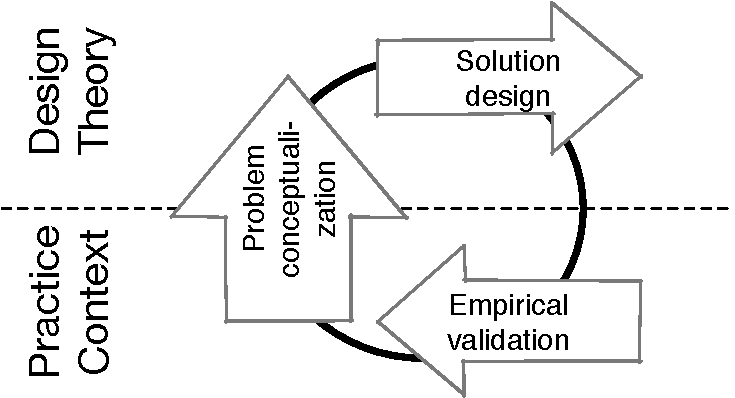
\includegraphics[width=0.6\textwidth]{Figures/DSSE_process.pdf}
% figure caption is below the figure
\caption{A visualization of the types of research activities that take place in design science research. These activities may be instantiated in different ways.}
\label{fig:DS_process}       % Give a unique label
\end{figure}


% Problem conceptualization
Design science research aims to address real practice problems, and thus \emph{problem conceptualization} is a core constituent of the research. This is typically, but not necessarily, the first step in a design science research endeavor. Understanding a general problem in terms of one or more concrete problem instances is a basis for understanding how this general problem may be solved. During the exploration of a specific problem instance, it may become clearer what the core of the problem is, thus focusing the potential solution design to these areas. 

% Towards solution design
While problem conceptualization is a basis for the research activity, it is not a pure description of the problem. Under the design science paradigm, problems need to be conceptualized in terms of an envisioned solution. Thus, problem conceptualization is often intertwined with the creative activity of \emph{solution design}, where alternative solutions and previous research are considered. 

% Validation
 The primary goal of \emph{empirical validation} is to assess whether the solution proposal is feasible for the problem instance. The scope of the design knowledge gained in a study can be extended by systematically extending the scope of the validation in subsequent studies. Thereby, the knowledge base of the research area is extended. 

Design science is a paradigm used in many different research fields and it is instantiated in many different variants. The above summary reflects what we have found prevalent in software engineering. Some of our rationale and alternative instantiations are discussed below.


\section{A Model of Design Science Research}
\label{sec:DesignScienceResearch}

\begin{figure}[t]
\centering
 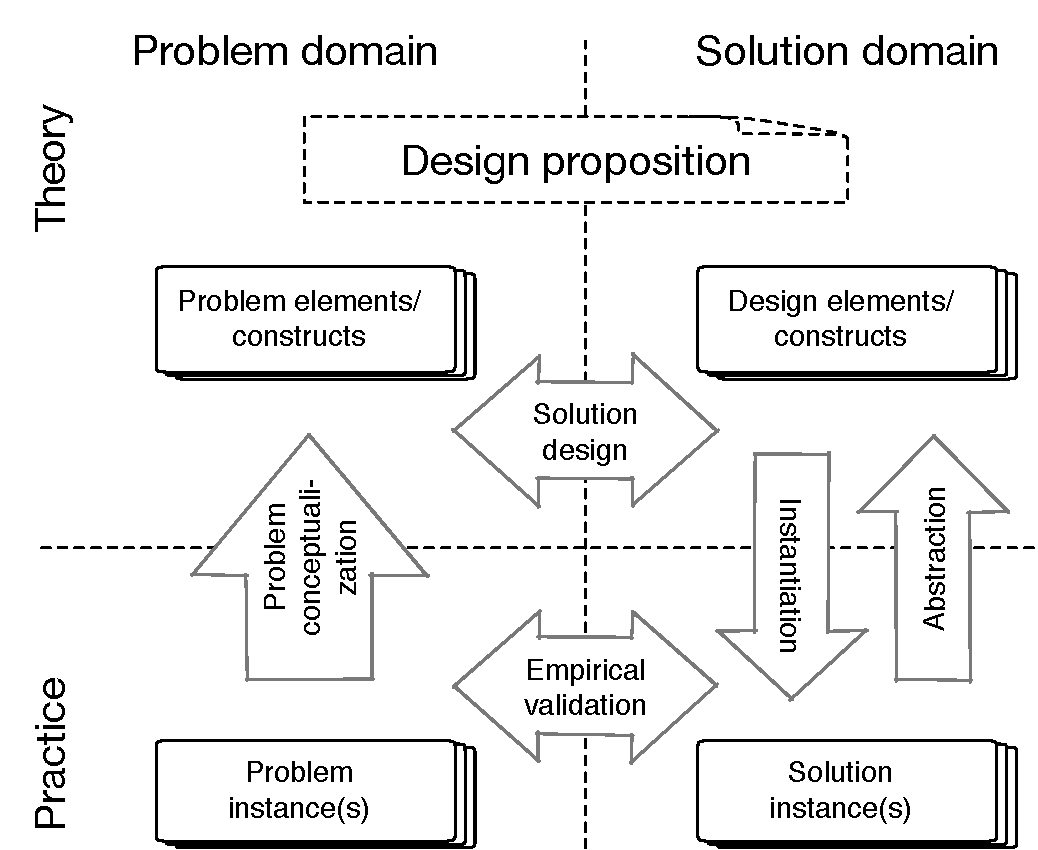
\includegraphics[width=0.8\textwidth]{Figures/DS_model.pdf}
% figure caption is below the figure
\caption{Model of design science contributions in software engineering~\cite{Engstrom19arxiv}. The boxes represent theoretical and practical \emph{contributions} of design science research, and the arrows represent \emph{knowledge creating activities} that can be performed by both practitioners and researchers.}
\label{fig:DS_model}       % Give a unique label
\end{figure}

% Description of the core of the model
Design science spans two major dimensions: the \emph{problem--solution} dimension and the \emph{theory--practice} dimension. To guide our in-depth elaboration of the design science paradigm, we extend the research activities model (Figure~\ref{fig:DS_process}) with design science contributions, see Figure~\ref{fig:DS_model}, where research activities under the design science paradigm can be expressed as transitions across this two-dimensional space.

% Semantics of the model
The \emph{practical} contribution of the research (i.e., the actual problem solving) is visualized by the boxes in the two bottom quadrants as instances of both the \emph{problem} and the \emph{solution}. The \emph{theoretical} contribution (i.e., generalization and scope definition) is visualized in the two top quadrants in terms of the \emph{technological rule(s)} and their \emph{constructs}. 
% Core consituents
The arrows in Figure~\ref{fig:DS_model} illustrate knowledge creating activities that can be performed by both practitioners and researchers. 
\begin{itemize}
\item \emph{Problem conceptualization} refers to the activity of describing the problem; % in terms of the envisioned solution; 
\item \emph{Solution design} refers to the activity of mapping a problem to a general solution; 
\item \emph{Abstraction} refers to the activity of identifying the key design decisions for a defined scope of validity of a solution; 
\item \emph{Instantiation} refers to the activity of implementing the solution in context; and 
\item \emph{Empirical validation} refers to an evaluation of how well the implemented solution addresses the problem.
\end{itemize}

%\per{Mention artifact? See reviewer 2}
These activities are performed iteratively across the theory--practice and problem--solution dimensions. Below we explore the contributions and activities of the design science model. 

\subsection{Technological rules and its constructs}
\label{sec:technologicalrules}

\per{Merged technological rules and constructs sections. Ok?}
% outline: The technological rule is the theoretical contribution of design science research also referred to as design knowledge.
A technological rule captures generalized knowledge about mappings between instances of problems and solutions (i.e., in-context validations), and thus is a means to transfer knowledge between contexts. The technological rule spans both a problem domain and a solution domain, and is formulated based on constructs in both domains. 

The scope of validity of the solution is described in terms of a  \emph{desired effect} of a \emph{proposed intervention} in a particular \emph{context}. Thereby, it frames the research outcome in terms of effects of interventions, rather than in terms of a solution to a problem. A technological rule can typically be expressed in the form: 
% outline: It can typically be expressed as: 'To achieve <desired effect> in <context> apply <intervention>

\begin{quote}{\emph{To achieve \textless Effect \textgreater ~ in \textless Context \textgreater~apply \textless Intervention\textgreater}.} 
%\newline
\end{quote}
The design knowledge within the technological rule aims to help software engineering professionals design customized solutions to their specific problems. Ideally it is a general recommendation based on current state of art, including new research contributions.

The notion of technological rules comes from Bunge~\cite{bunge_philosophy_1998}, while different instantiations of design science name the theoretical contributions differently. Gregor and Hevner discuss them in terms of design theory~\cite{gregor_positioning_2013}, Wieringa defines them as ``theories of artifacts in context''~\cite{wieringa_design_2009}. A thorough reflection about the role, nature and need for  technological rules in design science research is provided by van Aken~\cite{van_aken_management_2004}. 

% Generalization 
In a technological rule, a class of software engineering problems are generalized to a stakeholder's desired effect of applying a potential intervention in a specified context. 
Making this problem generalization explicit helps the researcher identify and communicate the different value-creating aspects of a research study or program.

%Examples of DS in SE
How the intervention in a technological rule is formulated may vary. It could, for example, refer to the use of a tool, articulate abstractions of the knowledge embedded in the tool, or even advice not to use the tool.
It could also refer to the application of a practice, a technique, a framework, or a set of guidelines. We extracted 38 examples of technological rules from a set of distinguished ICSE-papers from 2014--2018~\cite{Engstrom19arxiv}; these examples demonstrate the breadth of knowledge that can be represented using technological rules. These technological rules are available online at \url{http://dsse.org}.

% Hierarichical technological rules
One single instance of a problem--solution pair can generate multiple technological rules that are hierarchically related to each other. For example, an abstract rule may recommend using a general type of technology, while several more detailed rules may specify the use of technology, embedded in a specific tool. Similarly, there are hierarchical relationships with prior related technological rules to which a specific contribution is compared.
However, technological rules expressed at a very high abstraction level (e.g., ``To produce software of high quality, apply good software engineering practices'') tend to be either trivial or too bold (easy to debunk), while rules at very low abstraction levels have a narrow scope, and thus lack relevance for most software engineers. 

Thus, it is important to explicitly formulate the technological rule when presenting design science research and to be consistent with it, both when arguing for its relevance and its novelty, as well as when presenting the empirical (or analytical) support for the claims. A research contribution may refine any of the three constituents of an existing technological rule, add empirical support for the rule as a whole, or present a new rule.


% Constructs as theoretical design knowledge
Another type of theoretical knowledge produced in design science is the 
constructs on which we build technological rules. That is, the conceptualization of the problem domain and the solution domain, respectively.  
A construct can, for example, be a taxonomy that is used to articulate a technological rule or classify a set of technological rules in a research review. 
Taxonomies provide the means to relate different technological rules to each other. The different constituents of a technological rule may belong to different taxonomies. A construct can also be a conceptual model or a conceptualization approach that helps describe a problem in terms of an envisioned solution.

\subsection{Problem conceptualization and solution design}
 % Who, What, Where, When, Why and How

% (Who?) Problem understanding is ultimately an act of the practitioner but could be done in collaboration between researchers and practitioners or by researchers alone

In a mature research field, existing theory may help practitioners design solutions for their specific problems. Problem conceptualization is then an act of the practitioner, as is the instantiation of the solution in a specific context. In fields where the theoretical foundation is less mature, such as software engineering, researchers and practitioners may work together to advance and extend the scope of the theory. 

 Above, we described how design knowledge is first obtained and later matures through observations of real-life instances of problem--solution pairs. For each such instance, the problem needs to be formulated (understood) according to a conceptual lens. Such problem conceptualization can take place in collaboration between practitioners and researchers in, for example, action research or case study research, or by researchers observing software engineering practice.

% (What?) The outcome of the problem understanding step is a conceptualuzation of the problem instance towards an envisioned solution and thus tightly connected to a specific design approach

The outcome of the problem conceptualization is expressed in terms of problem constructs, matching corresponding constructs of an envisioned solution. If, for example, the proposed solution is to design a visualization system, the problem should typically be described in terms of a group of target users, their questions and tasks, and their measurements or data~\cite{meyer_nested_2015}. Thus, the problem contextualization is tightly connected to the solution design and cannot be performed in isolation. 

% (What?) The research contribution is not the conceptualization, but the identification of the problem instance (empirical support for prevalence of a conceptual problem) and potential updates of the modelling approach (new aspects of the technological rule)

% (When?) Problem understanding is the first step towards a solution design.

%Problem conceptualization is the first step towards a solution design. 
Depending on the type of solution, problem conceptualization may need to be repeated at several abstraction levels, starting with the stakeholder's problem description and, in case of a tool, reaching to the level of implementation details (such as choice of algorithm). If this is the case, different types of technological rules are used and validated at different abstraction levels. It is important to be aware of what these technological rules are, and to ensure that the validation of a solution takes place at all these levels and that the validations are mapped to the correct technological rules. Further, while solution design is a creative activity, the design knowledge it produces can be made more accessible and trustworthy if critical design decisions are clearly reported together with considerations about alternative solutions.

Finally, problem conceptualization is, to a large extent, in the eye of the beholder. A behavioral scientist would, for example, make a different problem conceptualization of a software project, compared to a software engineering researcher. Similarly, different software engineering researchers may be influenced by their background, emphasizing how problem conceptualization is intertwined with solution design.

 

\subsection{Validation, instantiation and abstraction}

To validate a technological rule it must be instantiated, preferably in multiple cases of problem--solution pairs that instantiate the rule where each case adds to the validity strength of the rule. Alternatively, a new technological rule may be abstracted from an observed implemented solution applied to a real-life problem.
The constituents of the technological rule implicitly specify the validation activities if expressed in the form of:

\begin{quote}{\emph{To achieve \textless Effect \textgreater ~ in \textless Context \textgreater~apply \textless Intervention\textgreater}.} 
\end{quote} 
The \emph{intervention} is the object of the validation study, the \emph{context}  refers to where the research is conducted, and the expected \emph{effect} defines the validation criteria. This points to real software engineering contexts as the ultimate validation context for design science research. 
Consequently, multiple case studies are brought forward as the natural research methodology in design science~\cite{van_aken_management_2004}. However, for some design problems, the characteristics of the real context may be very similar to the artificial context settings for the validation. For example, a tool which has no human--tool interaction can be evaluated with real or realistic data in an offline setting. In other cases, practical and economical limitations can prevent the research endeavor from taking place in real operational environments, and thus scaled down validation contexts may be used in the research. 

The risks related to validating interventions in business critical contexts may be high. If the intervention does not deliver the effect as expected, the outcome of the software engineering activity as a whole may be endangered. Furthermore, the costs related to implementing the intervention may also be high (e.g., changing a work flow or adapting the information infrastructure to a new tool). Thus the validation procedures should gradually extend the validation scope for the intervention to manage these risks.
However, reducing the scope and complexity of the validation context too much may reduce the realism, which is essential for addressing a relevant problem with a feasible solution. Studies in artificial contexts may be useful to validate specific mechanisms, but they are not feasible for complex systems studies.  

Stol and Fitzgerald adapted Runkel and McGrath's framework for research strategies to guide balancing generalizability, precision and realism in designing validation studies~\cite{StolABC18}. This framework may be useful in choosing research strategies in relation to the goals of the research endeavor. The framework defines two dimensions: 1)~universality/specificity of context and systems, and 2)~level of obtrusiveness, which have to be balanced, as discussed above. 

The specific choice of methods for the validation depends on the research question. Easterbrook \emph{et al.} provide guidance to the selection of methods for types of research question and conclude for the philosophical stance behind design science: ``Pragmatists use any available methods, and strongly prefer mixed methods research, where several methods are used to shed light on the issue under study.''~\cite{easterbrook_selecting_2008} 
This recommendation fits well with the design science paradigm and its pragmatist viewpoint.

\begin{figure}[t]
  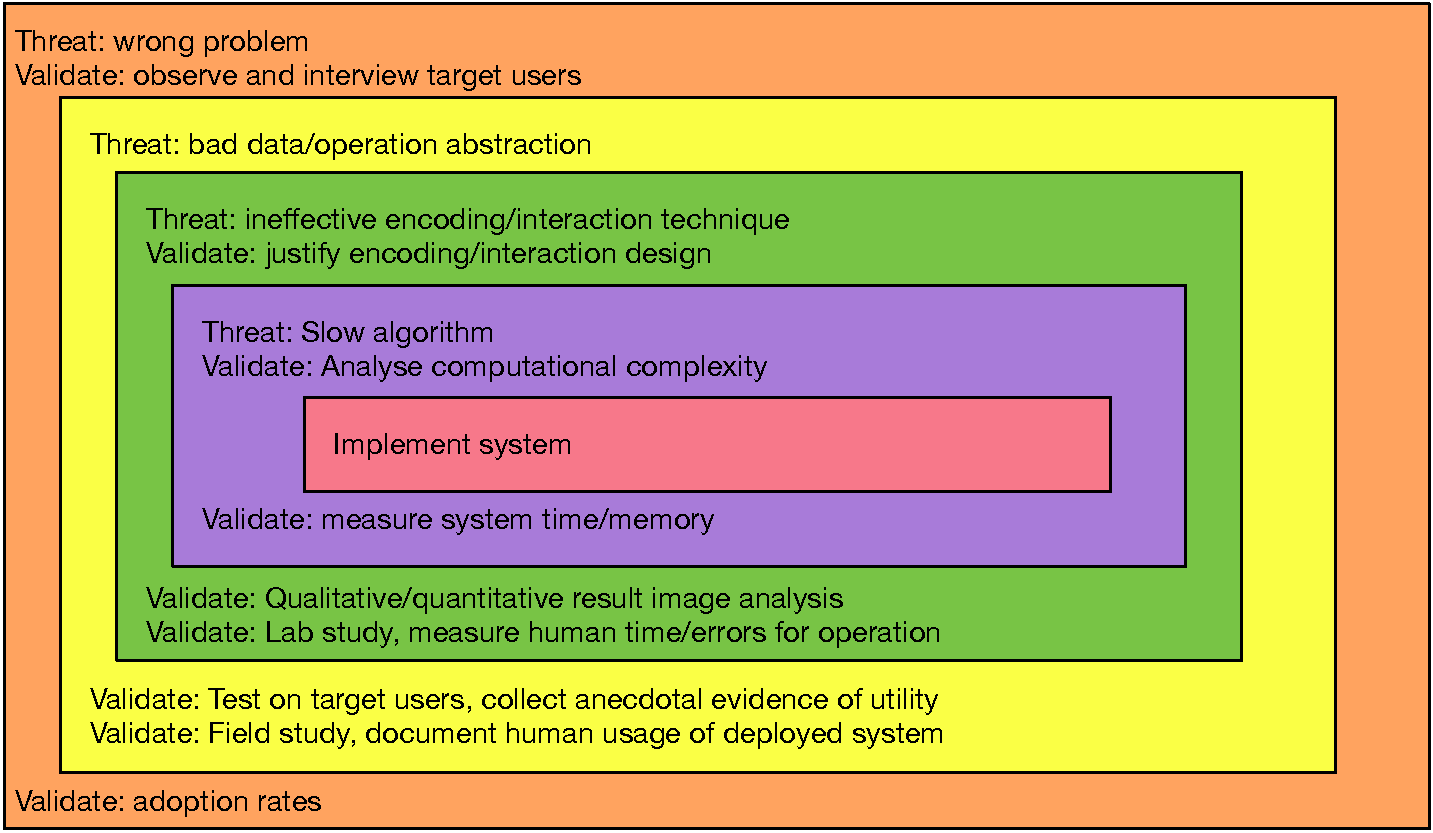
\includegraphics[width=\textwidth]{Figures/nested_model.pdf}
% figure caption is below the figure
\caption{Nested model for visualization design and validation~\cite{munzner2009}. At each level there is a ``black-box'' to be tested. Above the box, validity threats are specified and examples of validation strategies for the problem conceptualization are proposed for that abstraction level, while validation strategies for the instantiation of the solution are proposed below the box.}\label{fig:nested_model}       
\end{figure} 

Furthermore, the choice of validation method depends on the abstraction level of the validation. Munzner illustrates this in a nested model for visualization design and validation, see Figure~\ref{fig:nested_model}. This model shows how one design science project must respond to validity questions at several levels of abstraction, and that it is important to be consistent when selecting validation methods to avoid a mismatch between levels. As discussed in Section~\ref{sec:technologicalrules}, technological rules may be defined at all these different levels, and the scope of validity of each technological rule is defined by the context in terms of the conceptualization of the problem at the current abstraction level.

The design science paradigm primarily builds on theoretical/analytical generalizations, in contrast to explanatory sciences, which mostly rely on statistical generalizations~\cite{Runeson12Case}. Extending the scope of validity for a technological rule (i.e., creating a new, more general technological rule) is done by applying the intervention to new contexts, or by reasoning about the validity to another context by comparing key characteristics of the contexts. This is referred to as case-based generalization~\cite{wieringa_six_2015}.  
Technological rules may also develop from the general to the specific. The research may start with a general technological rule which is refined as new knowledge is gained through the instantiation of the technological rule in multiple contexts. 


\subsection{Design Science Research in Practice} 
\peggy{I like the discussion in this section a lot but it doesn't match the title very well...  perhaps this should go later in a discussion section or even earlier? I'm not sure... perhaps this could even go in further reading... or maybe the title should be about alternative views or something...}\per{Proposed title change}

The design science paradigm may embrace the use of a multitude of research methods. For \emph{problem conceptualization} and \emph{validation} of technological rules, empirical research methods are used, however, methods supporting natural settings are preferred as the problem in context is a focus for design science research. 

Design science is considered a methodology by other scholars in software engineering research~\cite{Wohlin2015}. As a consequence, they focus on the %valid research 
activities (how to conduct the research) rather than on the theoretical contributions of the research (how to theorize from the research), which is the case when it is considered a paradigm. However, %since a paradigm includes the methodologies, as defined above, 
there is a strong connection between the paradigm and the methodologies used.%, although the mapping is not one-to-one.

In a survey of 101 industry--academia collaboration projects, Garousi \emph{et al.} found 75 that were characterized as case studies~\cite{Garousi2019}. Further, they note that ``industrial case studies usually apply either the `exploratory' or the `improving' type, or both, rather than other case study types (descriptive, explanatory)''. Methods for data collection and analysis can be selected from the rich plethora of options available for such studies, for example, interviews, focus groups, observational studies, archival data analysis, and software metric analysis. 


Action research is another way of producing and validating technological rules.  41 of the 101 industry--academia collaboration projects surveyed by Garousi \emph{et al.} were labeled as action research~\cite{Garousi2019}. However, action research does not explicitly aim to develop knowledge that can be transferred to other contexts, but rather to make a change in one specific local context. However, both Wieringa~\cite{wieringa_technical_2012} and Johannesson and Perjons~\cite{johannesson_introduction_2014} discuss action research as one of several empirical methods that can be used to produce design knowledge.


Gorschek \emph{et al.} define a ``model for technology transfer in practice''~\cite{GorschekSW2006} focusing on industry--academia collaboration, which has some elements of design science. The model, which prescribes conceptual steps in solving a problem in an industry--academia collaboration setting, has elements of problem identification and conceptualization. The design of solutions involve studying the literature (state of the art) and selection of a candidate solution. This solution is validated in three steps, in academia, statically, and dynamically, before it is released into operations. 

The elements of this model fit the design science frame, although it (by intention) focuses primarily on the intervention in the specific context rather than the generalized knowledge and technological rule, which are significant elements of design science research. Further, when the generalization of knowledge and iterative knowledge building is stressed, it becomes clear that industry--academia collaboration is not a one-way transfer of technology, but a mutual interaction between the two.


\section{Using the Design Science Frame in Software Engineering}
\label{sec:UsingDSinSE}


 We designed a \emph{visual abstract template} as a tool to analyze design science constructs in software engineering research  (Section~\ref{sec:VA_template})~\cite{StoreyESEM17}. We suggest three direct uses of the design science paradigm as a frame for software engineering research, which we illustrate through an example (Section~\ref{sec:examples}). First, it can help in assessing contributions in research, both for the research community and during the planning and design of a research project (Section~\ref{sec:assessment}). Second, design science, particularly the technological rule, can be used in knowledge building, synthesizing and advancing the theoretical knowledge in the software engineering field (Section~\ref{sec:knowledge}). Third, the design science frame may help in communicating research across the research community and with industry (Section~\ref{sec:communication}). 


\subsection{A template to highlight design science constructs}% in software engineering}
\label{sec:VA_template}

\begin{figure}[t]
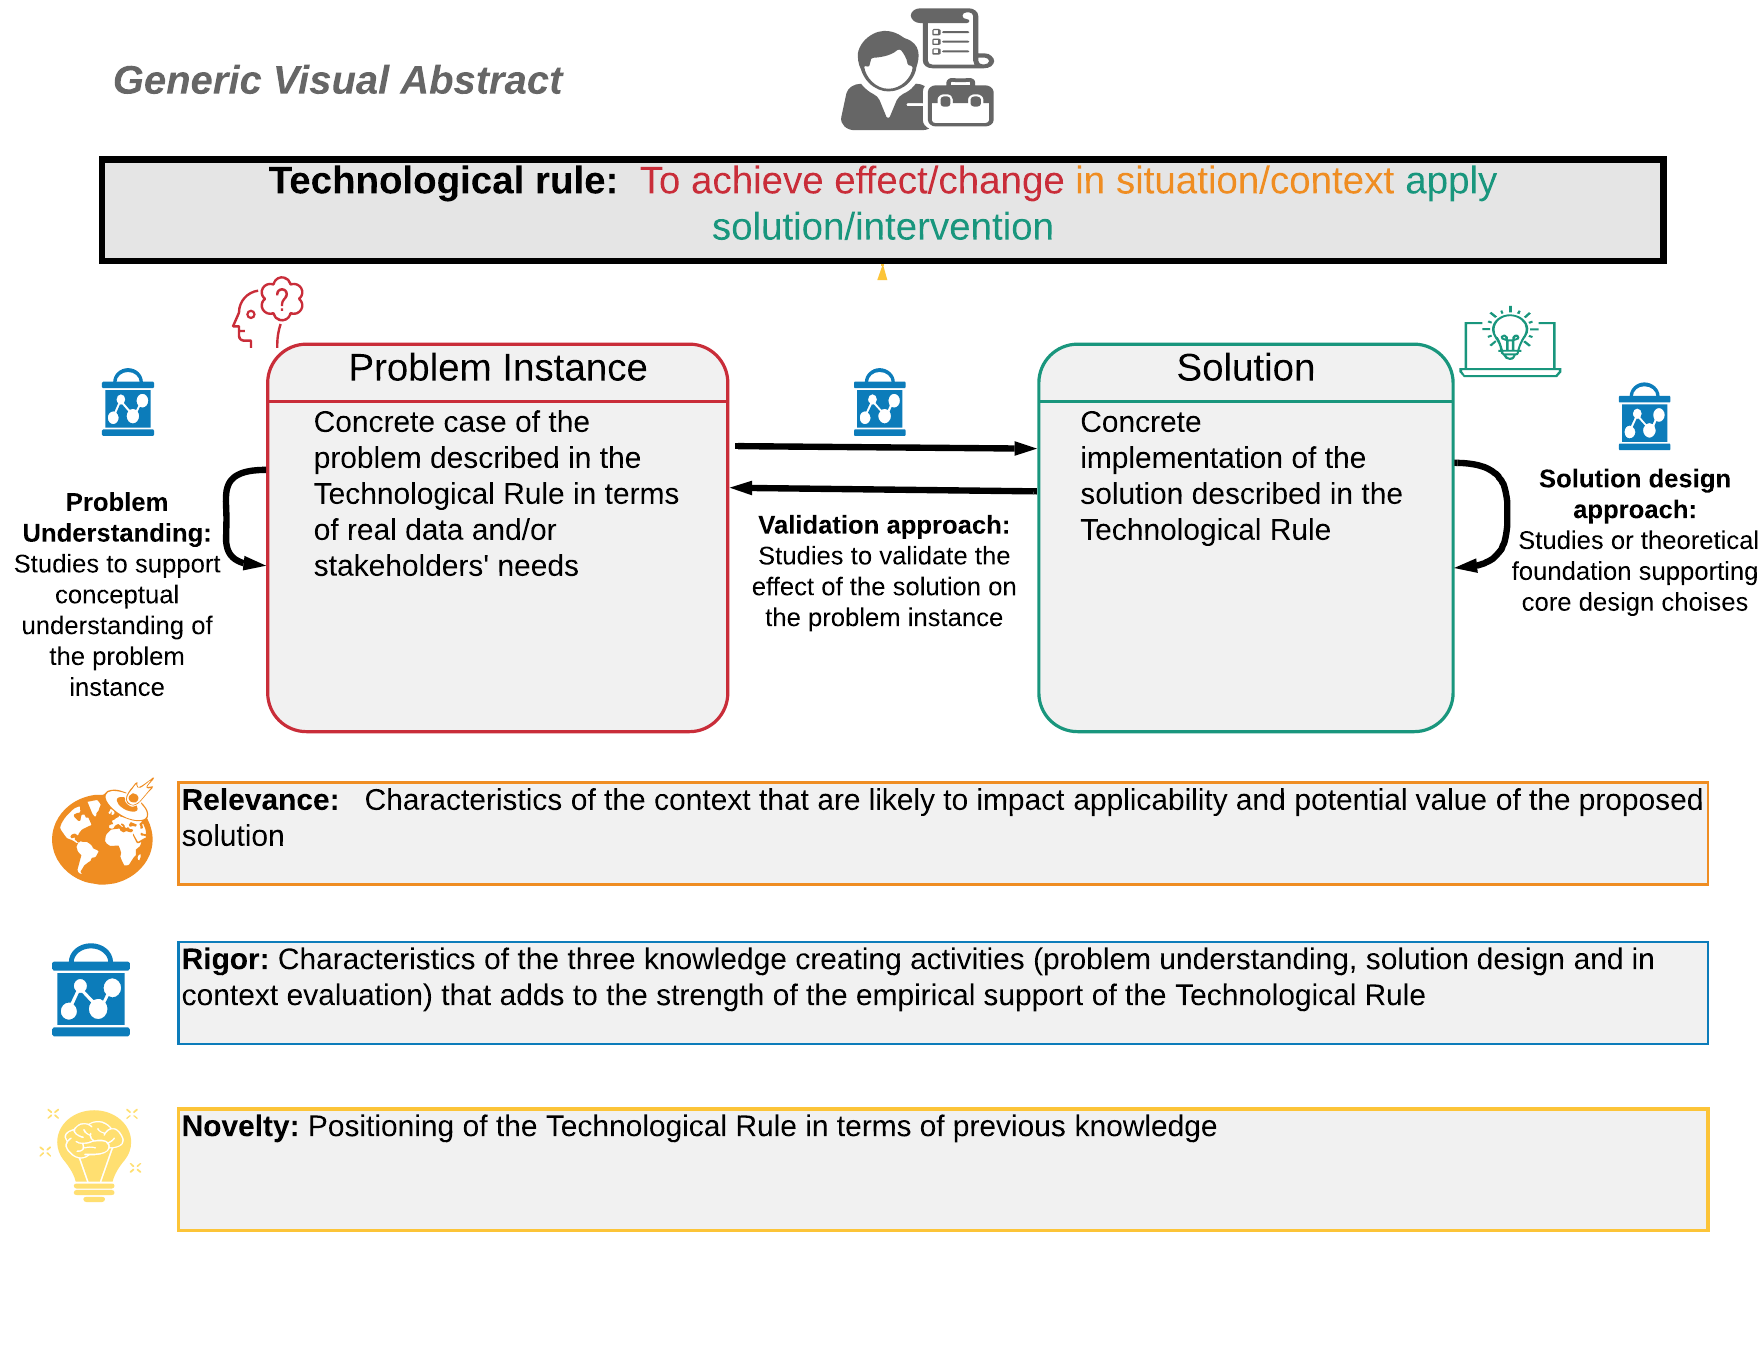
\includegraphics[width=1.0\textwidth, trim={0 15mm 0 0},clip]{Figures/GenericVA.png}
\caption{Visual abstract template including the core constructs in the design science paradigm.}
\label{fig:VA-template}      
\end{figure}


%Design Science as a Lens
The design science perspective is rarely used explicitly to design and present software engineering research~\cite{Engstrom19arxiv}. We therefore designed a \emph{visual abstract template} to help identify the design science constructs in software engineering research~\cite{StoreyESEM17}, see Figure~\ref{fig:VA-template}. We further extended the template with survey questions to help analyze software engineering literature from a design science perspective~\cite{Engstrom19arxiv}. The template aims to capture the key takeaway from a research study to help researchers assess the research contribution, build knowledge iteratively, and communicate research to practitioners. %Note connections to end of this chapter

Our design science template covers the main constructs of design science research: the theoretical contribution in terms of a \emph{technological rule}; its instantiation in terms of a real \emph{problem--solution} pair; the empirical or theoretical support for \emph{problem} conceptualization and the \emph{solution} design. Further, the bottom three boxes address the \emph{relevance} of the research, the \emph{rigor} of the research activities, and a statement about what makes the technological rule \emph{novel} in relation to the underpinning research, be it with focus on a refined problem conceptualization, or a new or improved solution design, or a validation of the the technological rule in a new context. 



\subsection{Design science example}
\label{sec:examples}
To illustrate the use of the design science lens for software engineering research, we present and discuss an example by Jonsson \emph{et al.}, introducing automated bug assignment to handle a large inflow of bug reports~\cite{JonssonBug15}. We have used the same example to illustrate our visual abstract~\cite{StoreyESEM17}, see Figure \ref{fig:BugAssignment}.

\begin{figure*}[t]
\begin{center}
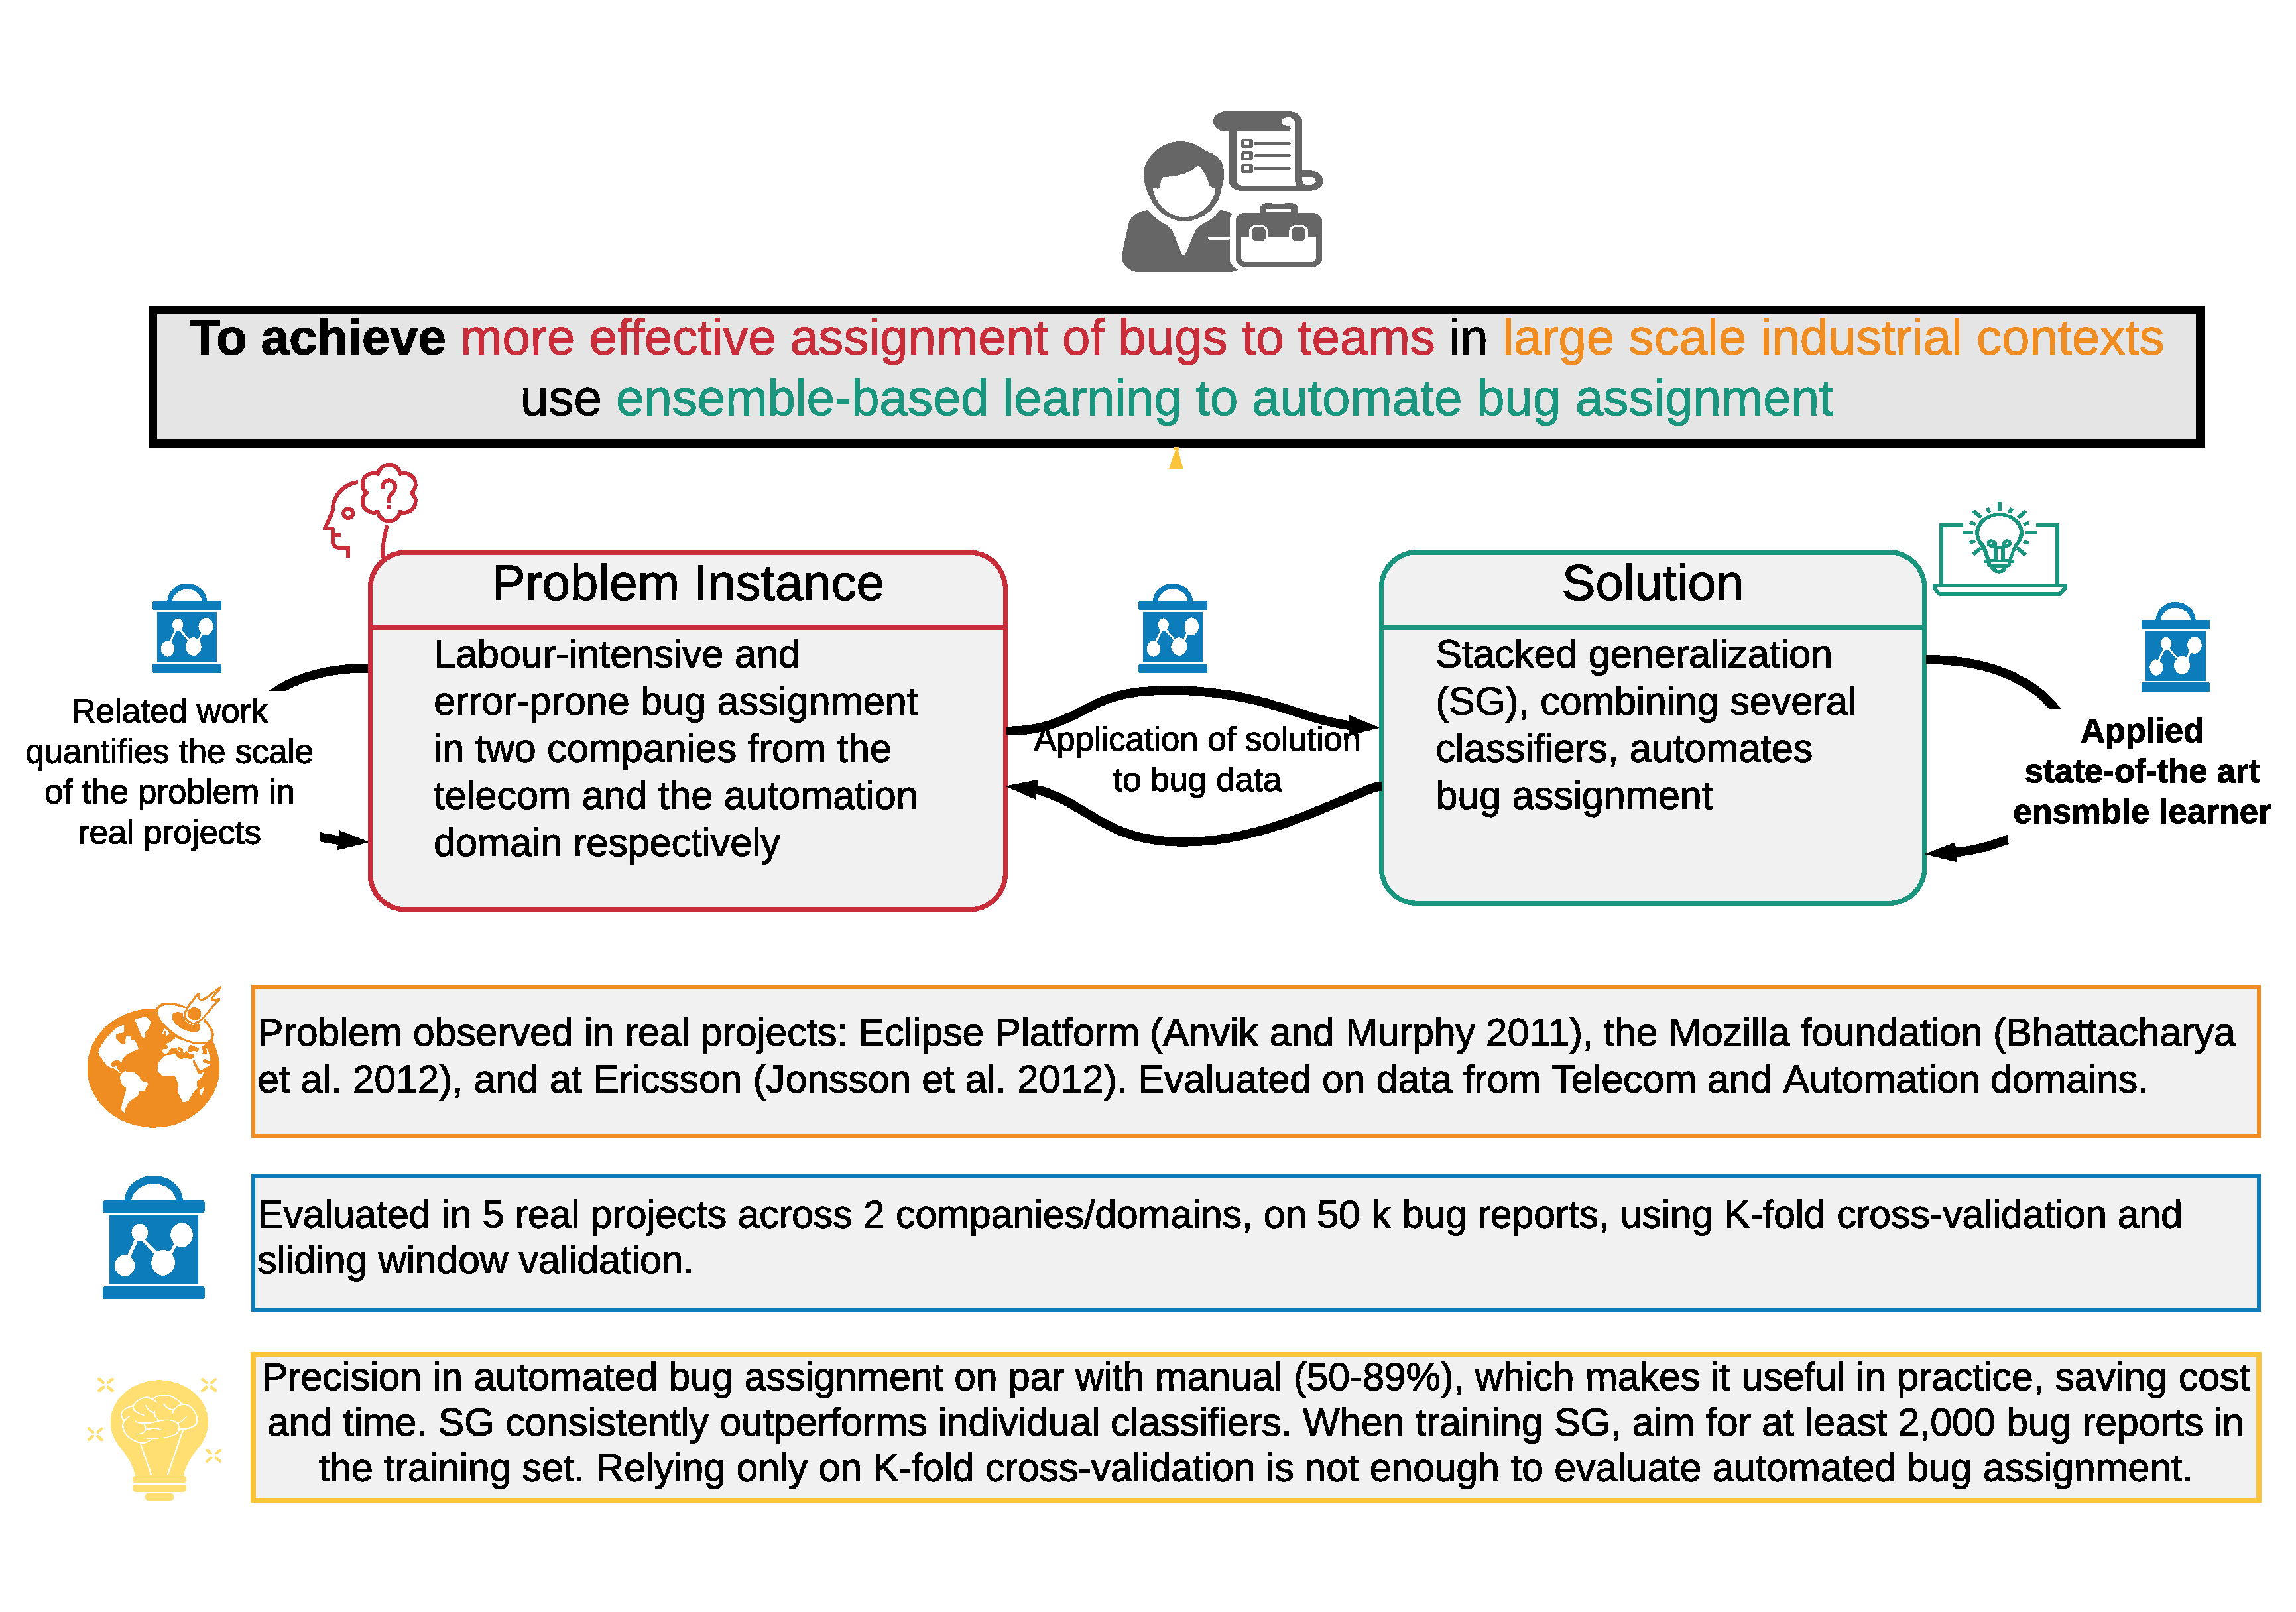
\includegraphics[width=\columnwidth, trim={5mm 20mm 5mm 20mm },clip]{Figures/VATemplateJonsson.pdf}
\caption{Visual abstract for the paper on automated bug assignment~\cite{JonssonBug15}.}
\label{fig:BugAssignment}
\end{center}
\end{figure*}

The automated bug assignment research was not originally presented within the design science frame. However, like much software engineering research, it is implicitly conducted as design science research~\cite{Engstrom19arxiv}. 
The scientific knowledge gained from the work can be phrased as a \emph{technological rule}:
\begin{quote}{To achieve more effective assignment of bugs to teams in large scale industrial contexts, use ensemble-based machine learning to automate bug assignment.~\cite{StoreyESEM17}}\end{quote}

The general \emph{problem} of inefficient bug assignment is observed in the literature as well as in the specific industrial contexts where this research was conducted. With the solution in mind (to use machine learning techniques to assign bugs to teams), the characteristics of the defect data and the organizational context were explored, and thus  identifying the characteristics of the \emph{problem instance}. Related work on bug classification as well as on machine learning techniques was identified~\cite{Borg2013EMSE}, which underpinned the \emph{design decisions} for the proposed solution. The machine learning solutions were implemented and trained using the Weka framework~\cite{hall_weka_2009}. Several alternative solution instances were \emph{validated} on real data (50,000 bug reports) from five projects across two companies/domains. For the specific companies, a design artifact was produced, namely the bug assignment tool built on top of Weka.



\subsection{Assessment of contributions}
\label{sec:assessment}

Hevner presents three research cycles in the conceptual model of design science, namely the \emph{relevance}, the \emph{rigor} and the \emph{design} cycles~\cite{Hevner2007}. We propose that the contributions of design science research be assessed accordingly with respect to \emph{relevance, rigor} and \emph{novelty}. 
Assessment of research contributions can be conducted proactively (when relevance may be a primary concern for consideration, and before the research is executed), prospectively (as the research is ongoing and when rigor should be carefully considered), or retrospectively (where novelty of the design knowledge produced may become more evident).
Below, we discuss assessments of contributions and refer to the example we described above.



% Peggy:  not sure what to do with this...
%\paragraph{Validation should be made in context and test the impact of the solution on the real problem}

\subsubsection{Relevance} 

%Relevance of a design science study is described in terms of problem similarity \peggy{similarity to what? oh I get it when I read it -- can this sentence be cut?} and solution applicability. 
The relevance of a research contribution can be viewed from two perspectives: 1)~from other practitioners that may benefit from the design knowledge produced, and 2)~from the research community. 

From an individual practitioner's point of view, the relevance of a research contribution may be assessed by comparing their specific context with the study context described in the research report. 
A practitioner may need to consider whether the design knowledge can be applied to their specific context as is, or if it should be customized in some way, or if the knowledge does not apply to their context or problem at all.
In the example by Jonsson \emph{et al.}, (see Figure \ref{fig:BugAssignment}) a practitioner, that faces the challenge of manually assigning bugs to teams, could benefit from using ensemble-based machine learning to automate bug assignment (or not). 

From the research community perspective, relevance is often considered in terms of how common the studied problem is, and how generalizable the produced design knowledge may be. These authors report 20 previous studies on machine learning-based bug assignment~\cite{JonssonBug15}, with different models for various bug report sets. To enable both types of assessments, relevant context factors need to be reported. Not all context factors are helpful in making this assessment, but only those that are critical for either the applicability of the solution or for the potential gain of applying the solution. 


\subsubsection{Rigor} 
Rigor of a design science study refers to the strength of the added support for the technological rule. It may be assessed in all of the three knowledge creating activities (problem conceptualization, design, and validation). 
Rigor should be considered when the research project is designed, as well as throughout and after the project to reflect on possible threats to validity. 
It is worth noting that the solution design activity is by nature a creative process and does not necessarily have to add to the rigor of the overall research. 

One aspect of rigor in the design activity could be the extent to which a solution builds on prior design knowledge, or whether alternative solutions have been taken into account. 
In the case by Jonsson \emph{et al.}, they choose alternative classifiers from the Weka tool by reasoning about their properties, and combined them into ensembles of classifiers for evaluation.

Rigor with respect to problem conceptualization and validation, are based on common empirical methods that support relevant validity criteria, such as using structured and transparent research methods and using realistic data. For example, the study by Jonsson \emph{et al.} can be considered high in rigor as the proposed solution is validated by its application to five defect datasets from two large software systems, comprising 50,000 bugs. Furthermore, they found that the precision in the automated bug assignment was on par with manual industry processes, which makes it scalable to practice.

\subsubsection{Novelty} 
Novelty of a design science study is expressed in terms of new or refined technological rules. Technological rules may be expressed at several abstraction levels, thus it is always possible to identify an abstraction level at which a research contribution is novel, may it be at the cost of general relevance. In the research by Jonsson \emph{et al.}, novelty of the intervention proposed in the technological rule is not straightforward to assess, as there already exists 20 studies on machine learning to automate bug assignment. The novel contribution here is the systematic design and evaluation of a machine learning approach, applied to a real-world context, as expressed in the technological rule.

However, novelty may not always be a priority in a given research effort.
To optimize rigor, novelty and relevance of reported research, one should strive to express the technological rule at the highest possible abstraction level at which it is novel, the provided evidence gives strong support, and the technological rule is not debunked by previous studies (or common sense). However, adding empirical support for existing, but under-validated, technological rules have a value of its own (replication), which makes novelty less important than the rigor and relevance criteria.


\subsection{Knowledge building}
\label{sec:knowledge}

Articulating the knowledge produced by our research in a more uniform way may help in building and synthesizing related knowledge in our community. 
The technological rules that emerge can at best be considered as theory fragments that prescribe and predict how a certain intervention for a particular context will lead to a proposed change. 
Our hope is that linking technological rules that are related (perhaps in hierarchical form) may help our community arrive at more general theories that can be refined and improved over time.

For example, Jonsson \emph{et al.}'s research on automated bug assignment is related to previous bug assignment research, although it is hard to compare due to a lack of detail and inconsistent (or lack of) phrasing of technological rules. If the contributions were clearly expressed as technological rules with corresponding validation, the outcomes together would be more generalizable.



\subsection{Research communication}
\label{sec:communication}

As we discussed above, building design knowledge in software engineering requires close partnership with practitioners. 
Practitioners may play a participatory role in our research by confirming and eliciting the problems to be solved, as well as by designing practical solutions using design knowledge and then validating them in context (on real problem instances). 
Consequently, how we communicate design knowledge to practitioners is critical to this participatory research approach.

We feel that technological rules will be valuable in communicating our findings to industry, and that the visual abstract may also appeal to those practitioners wanting to quickly gain a bigger picture of the research behind the design knowledge embodied by a technological rule. 
At the time of writing this chapter, we are in the process of evaluating our visual abstracts and in the future hope to evaluate them with practitioners.


Other initiatives for research communication include Petersen and Engstr\"om's framework SERP taxonomy architecture~\cite{petersen_finding_2014}, which includes the constructs of a technological rule  
%(i.e., desired effect, context and intervention) 
to support the mapping of practical problems with research. 
The SERP framework provides a taxonomy that establishes a common understanding between practitioners and researchers in software testing~\cite{engstrom_SERP-test_2017} and may support practitioners in their reviews of regression testing literature from a relevance point of view~\cite{ali_search_2019}, which may lead to generalized recommendations in terms of technological rules. 

Another attempt to make evidence available to practitioners is presented by Cartaxo et al.~\cite{Cartaxo2016}. 
They present the concept of ``evidence briefings'', which is a way to summarize systematic literature reviews in a one-page format. 
They used accepted information design principles to design the structure of the one-page briefing. The format and content were positively validated by both practitioners and researchers. While evidence briefings may provide an effective way to synthesize evidence from several studies, our visual abstract template provides a means to effectively summarize the contribution of one study or research program from a design science perspective.

\section{Recommended Further Reading}
\label{sec:reading}
Several fields of research have explicitly framed their work under the design science paradigm. This chapter is based on critically appraising these fields and adopting what we have found feasible for software engineering. We present the main literature sources and recommend them for further reading to advance software engineering under the design science paradigm.

Hevner has conceptualized design science for \emph{information systems research}, combining behavioral science and design science research~\cite{hevner_design_2004,hevner_design_2010}.
The philosophical stance behind design science is what is characterized as pragmatism~\cite{easterbrook_selecting_2008}, referring to a view that all knowledge is approximate and valued by its usefulness for solving practical problems. Hevner \emph{et al.} express this in terms of \emph{utility}: 

\begin{quote}
	That is the essence of design science. Contribution arises from utility. If the artifact does not solve the problem (search, implementability), it has no utility. If utility is not demonstrated (evaluation), then there is no basis upon which to accept the claims that it provides any contribution.~\cite{hevner_design_2004}
\end{quote}


Gregor and Hevner also refer to design science as a paradigm~\cite{gregor_positioning_2013}. Johannesson and Perjons  disagree with this view and argue that design science refers to the objective of changing the world---in contrast to describing it---and that this is done primarily by creating artifacts, not knowledge~\cite{johannesson_introduction_2014}. Johannesson and Perjons' view emphasizes design science as action research. Our stance is that design science is a paradigm for software engineering research, and as researchers our primary goal is to create knowledge to be applied by practitioners in the field. Furthermore, we consider artifacts as embedding design knowledge. 

Hevner adds three research cycles to the conceptual model of design science, namely the \emph{relevance}, the \emph{design}, and the \emph{rigor} cycles~\cite{Hevner2007}. The relevance cycle connects the environment with the design science activities, the design cycle iterates between designing and evaluating the interventions, while the rigor cycle connects the research with the theoretical foundation of the research. We were inspired by Hevner's work when we added assessment criteria to the visual abstract template.
%\peggy{I added this last sentence hope ok...}


Van Aken explored the design science paradigm for management science, with a focus on theoretical contributions captured as technological rules~\cite{van_aken_management_2004,van_aken_management_2005}. 
In the field of research with organizations as their study objects, van Aken proposed making a distinction between explanatory and design sciences by dividing the research into two fields: 
\begin{itemize}
\item Organization theory as description-driven research under the explanatory research paradigm, observing how organizations behave `naturally'; and 
\item Management theory as prescription-driven research under the design sciences paradigm, designing interventions to manage organization~\cite{van_aken_management_2004}.  
\end{itemize}

We do not propose a corresponding distinction for software engineering, but rather call researchers to awareness of the existence of these different paradigmatic perspectives and their implications on the choice of research methodology and knowledge building.

The Nobel Prize laureate in Economics, Herbert A.\ Simon, used other terms for the distinction between explanatory and design sciences paradigms~\cite{Simons69}. Design sciences are referred to as the ``science of the artificial'', in contrast to explanatory science as the ``science of the natural''. The latter refers not only to natural sciences in the narrow sense, but to other phenomena that seem to appear `naturally'. In this broader sense, we may find both `natural' and `artificial' phenomena in software engineering, and thus may frame the research in different paradigms depending on the phenomenon under study. 


Wierenga promoted design science for software engineering and information systems research in the concept of technical action research, including an engineering cycle and an empirical research cycle, which combine research with real-world consultancy projects~\cite{wieringa_six_2015,wieringa_technical_2012,wieringa_what_2014}. Further, to address the distinction between descriptive and prescriptive research, he introduces two types of research questions: \emph{knowledge} questions and \emph{improvement} questions~\cite{wieringa_design_2009}. He also discusses scaling up research to practice~\cite{Wieringa2014}. 

Munzner reviewed design science research in the field of visualization design and introduced a four-level nested model of design and validation, see Figure~\ref{fig:nested_model}~\cite{munzner2009}. She divides the design process into four distinct stages and emphasizes the importance of distinguishing between these levels when claiming contributions at more than one level. The nested model is a good example of a design construct in the solution domain, i.e., visualization, providing a lens for problem conceptualization. Although not all software engineering problems are solved with visualization approaches, the model may inspire similar thinking in other design processes. 


\section{Conclusion}
\label{sec:conclusion}
The design science paradigm is used in many fields of research that aim to understand and improve some area of practice. Software engineering researchers rarely use design science to frame their research explicitly, although our analysis showed that it resonates well with the aims of and research practice in software engineering~\cite{Engstrom19arxiv}. 

There are many flavors of design science in related fields of research. In this chapter, we propose an instantiation %\peggy{the word instantiation again -- I agree with it -- but it may throw some people off... but not sure how to replace it so let's leave it!} 
of design science that we find suitable for the characteristics of software engineering research. We also present our visual abstract template, derived to help assess and communicate design science research~\cite{StoreyESEM17}. 

We hope that the community will adopt the design science framework for software engineering research to provide better tools for researchers to define and assess relevance, rigor and novelty of research, to assist communication between researchers and with practitioners, and to support continuous theoretical knowledge building in software engineering. 


\bibliographystyle{plain}
\bibliography{dsse}
\end{document}
